\documentclass[12pt]{report}
\usepackage{graphicx}
\usepackage{algorithm}
\usepackage{algorithmic}
\usepackage{keystroke}
\usepackage{pdfcomment}
\usepackage{gensymb}
\usepackage{tabularx}
\usepackage{epstopdf}
\usepackage{url}
\usepackage[utf8]{inputenc}

\newcommand{\note}[1]{\raisebox{0pt}[0pt][0pt]{\pdfcomment[open=true]{#1}}}
\newcommand{\notedme}[1]{\note{#1}}
% [dme] reordered these document definitions - title, author, date -
% if they sit here, they can potentially use the macros you include
% from packages
\title{Avoiding the Dark Side}
\author{
        Leslie Chisholm \\
                Department of Computer Science\\
}
\date{\today}

\begin{document}
\maketitle


\begin{abstract}
\note{Algorithm listing is excellent, but mixing maths mode and algorithm a little bit more than ideal. Also all the labels aren't going to typeset correctly as written.}\note{unsure how to fix this}

\notedme{Thanks for the chapter title changes - I really do think they're better like you've made them! The same can be said for subsections like ``Sun'' though... ;-)}\note{ok I've changed the Sun subsection }

\notedme{Did the ``suburb'' masking code end up making it? I don't think the figures show anything but sun over the whole area. It would be great to have a table that shows a quantitive difference between Peninsula and North Valley sunlight over June, for example. Even if the code was nearly ready but not finished, it might be worth mentioning it, as being able to quantitatively compare the amount of sun between selected areas of the map would be a good extension.}
\note{It ``sort of'' made it in. To find the aggregate amount of sunlight a suburb receives you can mask out sections of map that are outside of the suburb and they won't be returned. Exporting this to a cvs file and taking the average sunlight of that area would be the ideal way to do it and could be compared to other sections. I've created a section in the aggregator describing comparisons between suburbs.}

\notedme{I didn't spell-check, but make sure you do before submitting it, obviously.}\note{Of course}

The hilly terrain and the low latitude of Dunedin, New Zealand causes varying amounts of sunlight throughout the city. This project set out to find the distribution of sunlight cast over areas of Dunedin at different times of the year and present this information in a usable manner. Collecting physical data of the Sun's position and geographical layout of Dunedin was integrated into a three-dimensional simulator and an accurate seconds-of-sunlight calculator, letting a user explore and witness how shadows change in real-time and accurately calculate the aggregate amount of sunlight an area receives over a period of time.
\end{abstract}

\tableofcontents
\listoffigures\
\listofalgorithms
\chapter{Introduction}
The city of Dunedin is well known for being a dark and cold city because of the hills surrounding the centre of the city that shade large areas in the winter months. This project set out to discover the amount of sunlight Dunedin receives over any given period of the year and present the data in a way that a user could visualise how the distribution changes over time and view the distribution of sunlight over a period of time.

\section{Goals}
The goals of this project were to research and implement a sunlight projection model for the city of Dunedin. There are two parts; an interactive three-dimensional display to show point in time distribution of sunlight over Dunedin and a data aggregator to augment the display with computed measures of sunlight coverage over time ranges.

\section{Chapter Outline}
This chapter introduces the project, its goals and gives some background information to the reader. Chapter two focuses on how physical data was gathered from the environment, the methods used to convert them into a representation usable for the project and the accuracy that was obtained in these measurements. Chapter three looks at the interactive three-dimensional viewer built to display the distribution of sunlight over Dunedin in real-time\footnote{Real-time is defined to be a program with a latency between frames of less than 40 milliseconds.} and its implementation using the Java OpenGL wrapper library~\cite{JOGL}. Chapter four is about the data aggregator, how it can accurately ray-trace the shadows by sacrificing the ability to run in real-time, the amount of sunlight an area receives, how the data it calculates can be explored and the results generated. Chapter 5 summarises how the project accomplished the tasks it set out to solve, the results of these tasks and remaining tasks that could be worked on.

\section{Background Information}
\subsection{OpenGL and JOGL} 
To create the viewer and allow it to be used in an interactive manner the Java OpenGL (JOGL)~\cite{JOGL} libraries are used. JOGL is a wrapper library that exports the OpenGL application programming interface (API) to the Java programming language. OpenGL or Open Graphics Library is a cross platform API for writing applications that use two and three dimensional computer graphics. The project uses version 2.0 of the OpenGL libraries for access to programmable shaders and buffer objects and will be able to run on any graphics hardware that supports OpenGL 2.0. Buffer objects are useful to store and retrieve data from the graphics card with little overhead.
OpenGL Shading Language (GLSL) programmable shaders are used to directly program the rendering pipeline to calculate large numbers of similar vector and matrix equations using the graphics hardware instead of the central processing unit.


\chapter{Physical Data}
To describe how shadows are cast over Dunedin, physical elevation models and mathematical models of the Sun's position are required. The digital elevation model is used to generate the three-dimensional map of Dunedin and the Sun's position is used to cast shadows over this map at given point in time. In this chapter the digital elevation model of Dunedin and the algorithmic model of the Sun's position will be described and checked for accuracy.

\section{Elevation Data}

\begin{figure}[h]
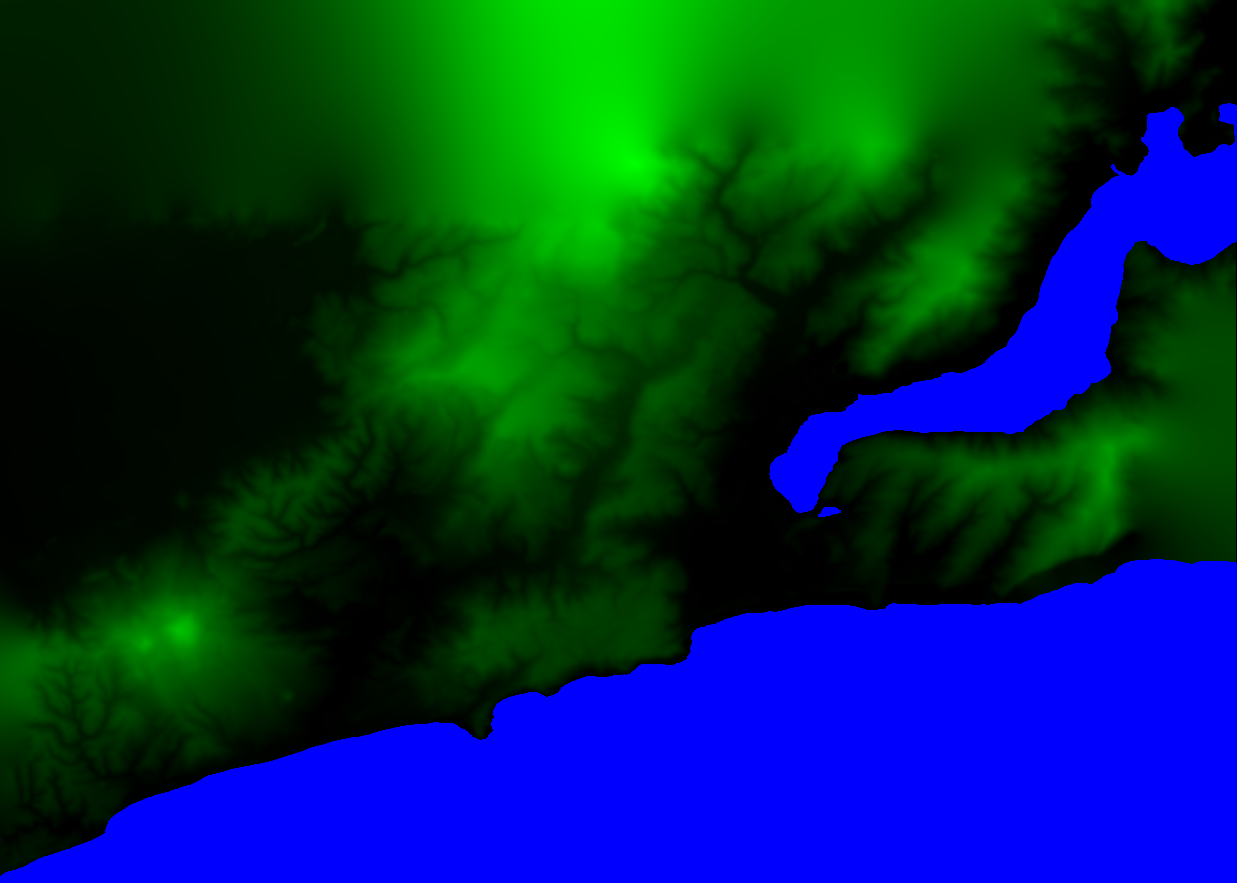
\includegraphics[width=\textwidth]{heightmapandwater.png}
\caption{A Height Map exported from the elevation data with areas of water painted in blue}
\label{image:elevation-water}
\end{figure}
The height data for Dunedin was collected from the surveying department of the University of Otago. The data contains a map with a width of 1237 points and a height of 881 points, with the $x,y$ data points separated by 15 metres and covers most of general Dunedin from South Taieri to the top of Pine Hill. The data is encoded as a 1237x881 text file of decimal pointed numbers that represent the height above sea level in metres at that point, where position $0,0$ is south-west of Brighton and $1237,881$ is slightly north of Port Chalmers. There are areas where the data is approximated that lie outside the urban area of Dunedin, such as the hills north of Halfway Bush and East of Highcliff.

\subsection{Height Points Below Sea Level}
The definition between the ocean and land is complicated when dealing with areas of reclaimed land like South Dunedin, where areas of land can be below sea level but not in the ocean. It was originally assumed that all areas of land below zero metres were in the ocean, however doing this caused large areas of reclaimed land around the harbour area to be in the ocean and was highly inaccurate when compared to a satellite image of Dunedin~\cite{gmaps}.To work around the lack of definition of what is below sea level and what is not, an image was generated (see figure~\ref{image:elevation-water}) with the areas of water coloured a strong blue (RGB 0,0,255). The image is overlayed on the height data map when being used in the viewer with a 1:1 mapping of height points to image pixels to represent the areas of land that fall into the ocean. Areas of the height data that fall in the water are clamped to a height of 0.1 because the shape and depth of the ocean floor is of no use to this project.

\subsection{Accuracy}
In the project proposal the accuracy of the height data was going to be checked using a global positioning system (GPS). Unfortunately after some initial testing and research it was found that the height returned by GPS device is rated to be accurate to approximately $\pm$ 15 metres 95\% of the time~\cite{gpsaltitude}. These inaccuracies were observed when standing approximately 2-3 metres above sea level \note{on a beach don't think I need to say this}\notedme{what about tides?}\note{the tide was 3/4 high} with a GPS and getting results 10 metres above sea level.

The best way to confirm the accuracy of the height data would be to compare it to other geographical data sources. Before going to the surveying department for the height information other sources were tried. The Shuttle Radio Topography Mission (SRTM)~\cite{srtm} was a near-global scale project by NASA to generate topographical maps and includes all of New Zealand at a resolution of 30 metres between data points. An old version of ARC GIS was provided by Geoff Wyvill containing topographical information of New Zealand, unfortunately the software used to read the topographical map information was old and could not be run in such a way to export the data. Scraping height data off Google Maps~\cite{gmaps} was attempted but the large number of HTTP requests required to collect a 1000 by 1000 map of Dunedin was impossible because of the limit on HTTP requests Google lets any single person perform.

\subsection{Future Work}
Integrating other height data that includes other cities and geographical regions was left out of the project because the main area of focus was the Dunedin region. Collecting a larger data set would allow for contrasts and comparisons between the aggregate amount of sunlight two areas receive and allow the programs to work on a more general level.

\section{Mathematical Model of the Sun's Position}
To generate shadows over the representation created of Dunedin the direction vector to the Sun at a given time has to be calculated accurately using a given time and geographical latitude and longitude. To calculate the position of the Sun, algorithms from the Redshift~\cite{redshift} software project were translated into Java and integrated into the project.

\subsection{Calculating the Position of the Sun}
To calculate the position of the Sun, the current Julian date, solar declination and hour angle must be determined. The Julian date is calculated by converting the current system time in seconds elapsed since January 1st 1970 to the current Julian Date in coordinated universal time (UTC) and days and fractions of days elapsed since January 1, 4713 BC. The hour angle is the angle between the plane of the Earth and the plane of the Sun at a given time and is zero when the Sun is directly above the Earth during solar noon. Calculating the hour angle can be done using the current longitude and Julian time. Solar declination is a measure of how many degrees north or south of the equator the Sun is when viewed from the centre of the Earth and can be calculated by the current time. By converting these calculations to the current latitude the Sun's current azimuth and elevation can be computed accurately.

Code from the open source Redshift project~\cite{redshift} was used to calculate the position of the Sun.  Code from other projects were examined, such as the solar positioning libraries for Java~\cite{javasunlib}, however the algorithms used in this library, the PSA~\cite{psa} and SPA~\cite{spa} algorithms, have the unfortunate downside that the algorithms they are based on do not work for areas in the Southern Hemisphere~\cite{southsun} and modifying these algorithms to work in the southern hemisphere is outside the scope of the project.

The code modified from the RedShift project to find the current solar elevation are the \texttt{solar.c} and \texttt{solar.h} files, which are based on JavaScript code by U.S.\ Department of Commerce, National Oceanic {\&} Atmospheric Administration~\cite{usnoaa} and is based on equations from Astronomical Algorithms~\cite{astronomicalalgorithms}. Code from the Redshift project is used to calculate the current Julian date, solar declination, hour angle and solar elevation. Calcuating the solar azimuth is not performed by Redshift so other methods of calculating it were explored. After trying many different algorithms, the only azimuth calculator that handled negative latitude and times when the altitude is 90{\degree} was the method described on the University of Southern California's Architecture Site~\cite{solarazi} that breaks the azimuth calculation down into the $x$ and $y$ components for greater precision.

\subsubsection{Time}
Calculating the position of the Sun requires the current time to be known. Java's built in GregorianCalendar class is used to keep track of the current date/time, handle changes in time zones and update the time automatically. The method \texttt{getSystemTimeMillis} is used to get the current time from the calendar when calculating the position of the Sun because it returns the current UNIX time in milliseconds which can then be passed to the Redshift libraries to calculate the Julian date. A purpose built Time class is used to keep track of and update the current time.

When the Sun goes down ( $\mathit{elevation} < 0$ ) the Time class's update method takes control from the program calling it and enters a loop that increments the time and recalculates the suns position, until the Sun comes back above the horizon. The time firstly jumps forward by six hours, because the shortest night in Dunedin is no less than 6 hours long, and is then incremented in one minute steps. Once the Sun elevation is greater than zero the time code breaks out of the loop and returns control back to the program. Taking control of the time once the Sun goes beyond the horizon prevents the program from doing unnecessarily calculations and ensures at every point in time the Sun is shining on some part of the map. 

Originally code for calculating the sunrise and sunset times was going to be used to calculate the amount of time that needed to be skipped before the Sun came back over the horizon. These calculations proved to be inaccurate, difficult to implement and unnecessary when compared to exhaustively searching for the next sunrise. The amount of time taken to exhaustively search for the next time the Sun is over the horizon took a very small amount of time (no more than 53 milliseconds and an average of approximately 5 milliseconds) and optimising it is unnecessary. A form of gradient descent to calculate the precise time of sunrise and sunset was explored but not implemented, again because the optimisation and accuracy gained was not needed.

\notedme{although presumably the next sunrise time could be determined in a closed form equation, or by some sort of method of descent.}\note{yes it could but the time it takes to exhaustively search is so little it is not worth it}\notedme{Yep, I understand that, but that's true for your particular application, and you can emphasise that in the text, but it's not a big issue anyway}\note{fixed and did some practical testing}
\subsection{Sun Accuracy}

\begin{figure}[h]
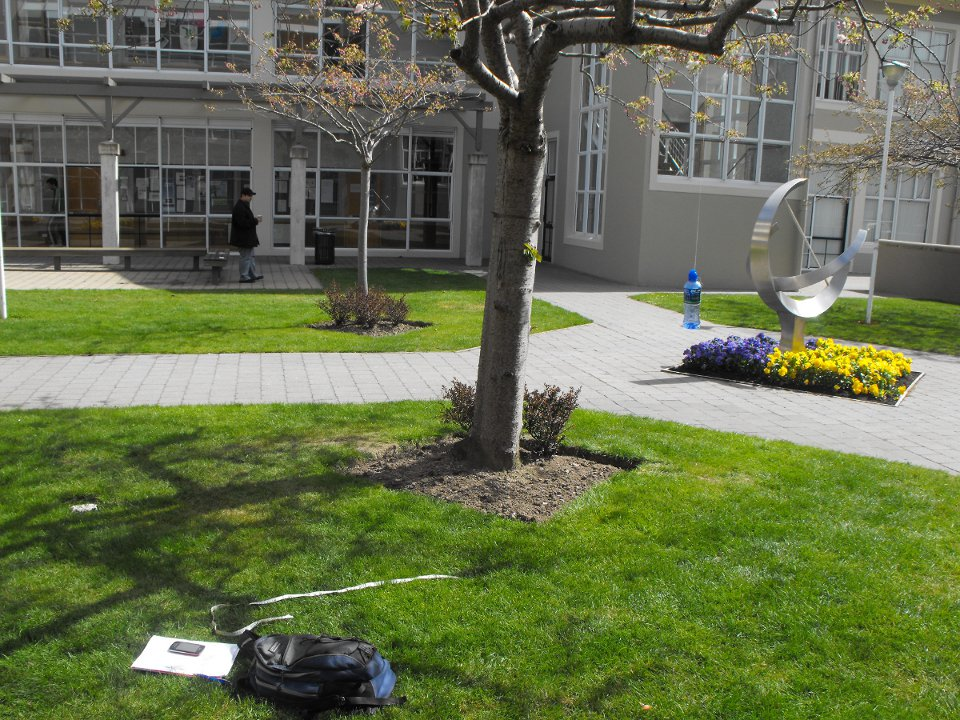
\includegraphics[width=\textwidth]{contraption.jpg}
\caption{Device used to approximately calculate the position of the Sun}
\label{image:sun-contraption}
\end{figure}

\begin{table}
{\small
\begin{tabularx}{\textwidth}{ | p{2.2cm} | X | X | X  | X |}
\hline
Time \& Date (2011) & Sun Azimuth Website & Sun Azimuth Project & Sun Elevation Website & Sun Elevation Project\\ \hline
09:30 1-Jan & 87.94462{\degree} & 87.9465{\degree} & 35.06{\degree} & 35.039{\degree}\\ \hline
12:00 7-Apr  & 12.54622{\degree} & 12.5412{\degree} & 36.77{\degree} & 36.74896{\degree}\\ \hline
16:00 14-Jun  & 314.4235{\degree} & 314.4227{\degree} & 7.243{\degree} & 7.1254{\degree}\\ \hline
14:00 18-Aug & 338.3437{\degree} & 338.34310{\degree} & 28.35{\degree} & 28.3225{\degree}\\ \hline
15:19 4-Oct & 321.1353{\degree} & 321.12823{\degree} & 41.72{\degree} & 41.698387{\degree}\\ \hline
\end{tabularx}
\caption{Calculated position of the Sun using data scraped from \url{satellite-caculations.com}~\cite{solarpos}}
\label{table:websun}
}
\end{table}

The accuracy of the Sun's position calculations were tested by comparing the results from the algorithms used in the project with results from other Sun position calculators and by setting up a physical experiment to calculate the position of the Sun. Using the solar position calculator from \url{satellite-caculations.com}~\cite{solarpos} the
 calculations were compared to the ones generated in the program. Observing table~\ref{table:websun} it can be seen that the results generated by the Sun algorithms in the project accurately resembles that generated by other calculations. Without taking atmospheric refraction into account and the accuracy obtained is more than enough for calculating shadows.

A rudimentary device seen in figure~\ref{image:sun-contraption} was used to calculate the physical position of the Sun. The azimuth can be found by measuring the angle between north and shadow and the elevation can be found by measuring the length of the shadows against the length of the device. The device is made up of a piece of string tied to a weight and is hung from above to ensure that the device is pointing towards the centre of the Earth. The azimuth was recorded using a magnetic compass on a mobile phone and modified to point to true north by applying Dunedin's magnetic declination (the angle between magnetic north and true north) of approximately 24.8{\degree} east. Data was taken from this device at three different times on the 5th of October from outside the Opheo building.

\begin{table}
\begin{tabularx}{\textwidth}{ | l | X | X | X | X |}
\hline
Time & True Sun Azimuth & Sun Azimuth Calculation & True Sun Elevation & Sun Elevation Calculation\\ \hline
13:08 & 15.8{\degree} & 7.027{\degree} & 44.09{\degree} & 48.4507{\degree} \\ \hline
14:47 & 344.8{\degree} & 330.967{\degree} & 40.376{\degree} & 45.1352{\degree}\\ \hline
15:12 & 337.8{\degree} & 322.955{\degree} & 43.914{\degree} & 42.766{\degree}\\ \hline
\end{tabularx}
\caption{Calculated position of the sun using real data taken on October 5th 2011}
\label{table:realsun}
\end{table}

From table~\ref{table:realsun} it can be seen that the calculation differences are quite different between the physical position of the Sun and the calculated position of the Sun. The difference is caused almost entirely by the errors in gathering the physical data and physical anomalies such as atmospheric refraction. Firstly, the mobile phone compass used to find the azimuth of the Sun is highly inaccurate giving values that were $\pm$40{\degree} for the same direction. Secondly, the device created to measure the elevation of the Sun had a tendency to oscillate in the wind, and lastly the surface on which the length of the shadow was measured was not perpendicular to the device. All of the elevation calculations are within 5{\degree} and the azimuth calculations are within 20{\degree} which is within the possible margin or error caused by these effects. Compensation for these errors is outside the scope of this project and thus it is safe to assume that the calculations performed to find the Sun's position are accurate enough for the shadow calculations.

\chapter{Three-Dimensional Simulation of Real-Time Shadow Information}

\begin{figure}[h]
\centering
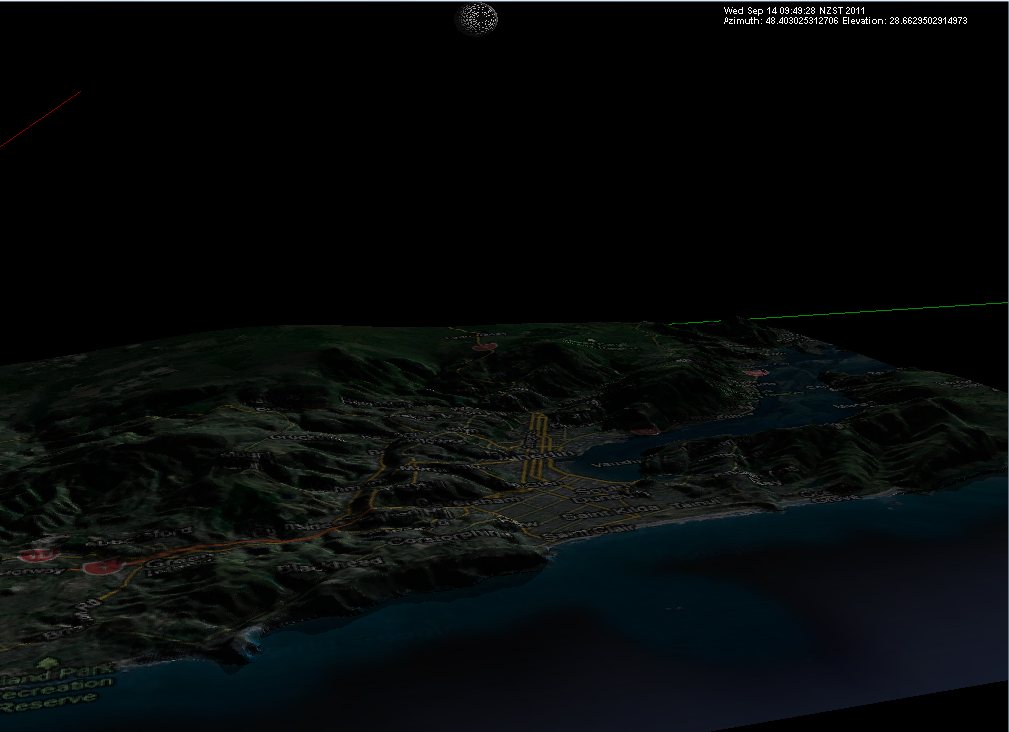
\includegraphics[width=0.8\textwidth]{viewer.png}
\caption{A screenshot of the viewer looking down at Dunedin}
\label{image:viewer}
\end{figure}

The viewer is an interactive three-dimensional simulator of the Sun as it travels through the sky over the city of Dunedin. It allows the user to view shadows cast by the Sun over the varying landscape in real-time. It exposes the ability to run in two different modes; shadow-mapping mode, where OpenGL shadow maps are used to generate shadows, and aggregator shadowing-tracing mode, where the shadow data from the aggregator is used to calculate shadows. Runnning the viewer in OpenGL shadowing mode allows the viewer to be used in real-time with less accurate shadows then those generated by shadowing-tracing the shadows. The user can control the position of the camera in the viewer, the current time and many other variables to see the simulated city from any perspective and time that the Sun is above the horizon.

\section{Drawing the Scene}

\subsection{Elevation Data}
Geographical height data is drawn by the viewer using OpenGL. After the height data has been decoded and stored in an internal data structure OpenGL buffer objects are created to store the vertex position, colour, texture coordinates and vector normals. Buffer objects allow storing of the vertex and texture data directly in the graphics card's local memory where it can be redrawn and updated quickly. Due to the large number of vertices present in the height data and the static nature of the data, using buffers to store the vertex data significantly lowers the number of draw calls to the graphics hardware, in comparison to using the fixed function pipeline, and decreases the amount of time between frames in the viewer. Once the vertex data has been passed to the graphics memory it is drawn onto the screen by passing it through a set of GLSL shaders to calculate the vertices final screen position and colour.

\section{Textual Information}
In figure~\ref{image:viewer} there is a box in the top right hand corner that shows the current time, solar azimuth and solar elevation. Drawing this information is useful because the current state of the time and solar position can be exposed to the user without leaving the viewer. Drawing this data is done using the built in JOGL TextRenderer class and is rendered over top of the final scene using a two-dimensional orthographic projection matrix.

\subsection{Overlay Data}
\begin{figure}[h]
\centering
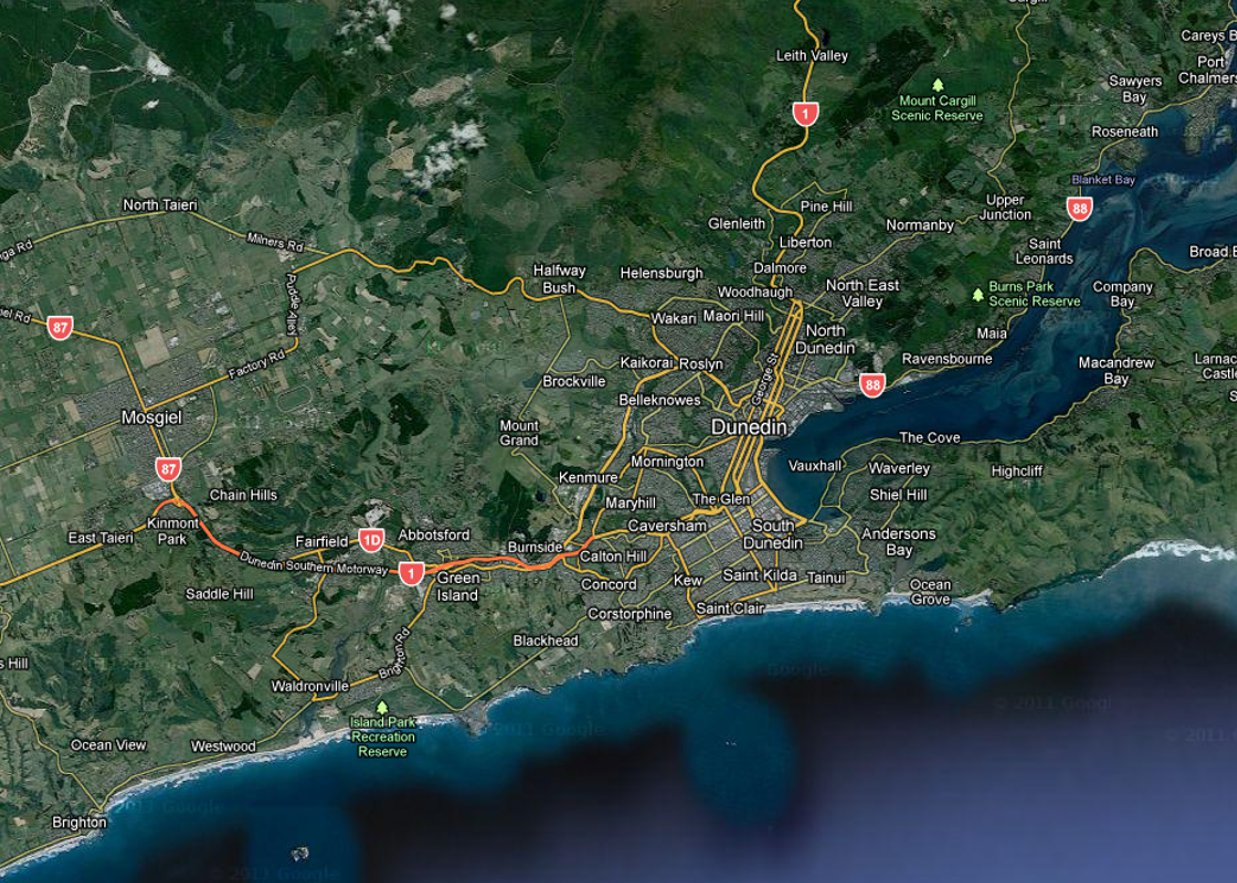
\includegraphics[scale=0.3]{suburbs.jpg}
\caption{Map overlay presented over the elevation data}
\label{image:overlay}
\end{figure}
A map overlay in figure~\ref{image:overlay} is drawn on top of the elevation data to show major roads, points of interest and terrain information. This gives the user an extra reference point to find specific areas that they may be interested in examining. The map was taken from Google Maps\footnote{This includes Google's copyright watermarks.} \cite{gmaps} and scaled to be the exact width and height of the height data. The overlay information is drawn into the scene by setting the vertex's material colour to be the colour of the overlay map at the vertex's $x,y$ position.

\section{Shadows, Lighting and Textures}
Shadows, lighting and textures are drawn onto the scene using GLSL vertex and pixel shaders. Diffuse and specular lighting are performed by calculating the dot product of the vertex normals with the direction vector to the Sun. Shadow lighting is implemented by using shadow mapping to test whether a given pixel can be seen by a light source. Textures are drawn in the fragment shader using the built in GLSL sampler2d data structure to store the pixel data and texture2D function to get the colour at a given vertex from the texture.\note{lowered density slightly}\notedme{?}\note{In your previous comment you said this section was a bit dense}

\subsection{Shadow Maps}
Shadow mapping is a method of quickly generating shadow information from a three-dimensional view which sacrifices accuracy for speed and ease of implementation. Shadow mapping works by storing the depth values of a scene from a lights point-of-view into an off-screen frame buffer and testing the depth component of each pixel in the scene against the stored depth value at that pixel in the buffer. If the depth buffers from the pixel are not present in the frame buffer than the point is said to be in shadow and is dimmed. In implementing shadowing mapping , OpenGL and GLSL shader code code was copied from Fabian Sanglard's website~\cite{shadowb} and modified from C++ and GLUT to work using Java and JOGL.

\subsubsection{Rendering the Scene From the Sun's Position}
The position of the Sun is drawn onto the scene for reference purposes as a OpenGL Utility Toolkit (GLUT) sphere and is calculated by fixing the distance from the scene to the Sun to be 15 kilometres. From this position the scene is rendered into the off screen frame buffer using an orthographic projection matrix. If the sun is placed far away from the scene the resolution of the shadow map suffers because the frame buffer contains areas that are outside of the scene and are not being utilised. Using an orthographic projection matrix allows the scene to be drawn close to the scene, while still lighting all points that would be seen if the sun was infinitely far away from the scene.

\subsubsection{Shadow Map Accuracy}
The accuracy of a shadow map is limited by the resolution of the off-screen buffer and the accuracy of the depth buffer. The resolution of the shadow map used in the viewer is 8 times that of the scene and so is reasonably accurate at the expense of some speed. By making the resolution of the shadow map larger the artefacts generated around the edge of objects is reduced, for example when the Sun is low on the horizon increasing the resolution of the shadow map reduces the amount of jagged edges at the intersection between areas in shadow and areas not in shadow. 

Increasing the precision of the depth buffer reduces self shadowing, which can be seen occurring around the tops of hills in figure~\ref{image:aggregatorvsshadowmapping}. A small hack is used in the shadow mapping code to decrease the amount of self shadowing by increasing the height of the depth buffer by a small (0.005) value, unfortunately it does not remove it entirely and increasing the precision of the depth buffer would requires less vertices to be drawn onto the scene or suffering a performance penalty.

\section{Visual Comparison Between the Viewer and Dunedin}
\begin{figure}[h]
\centering
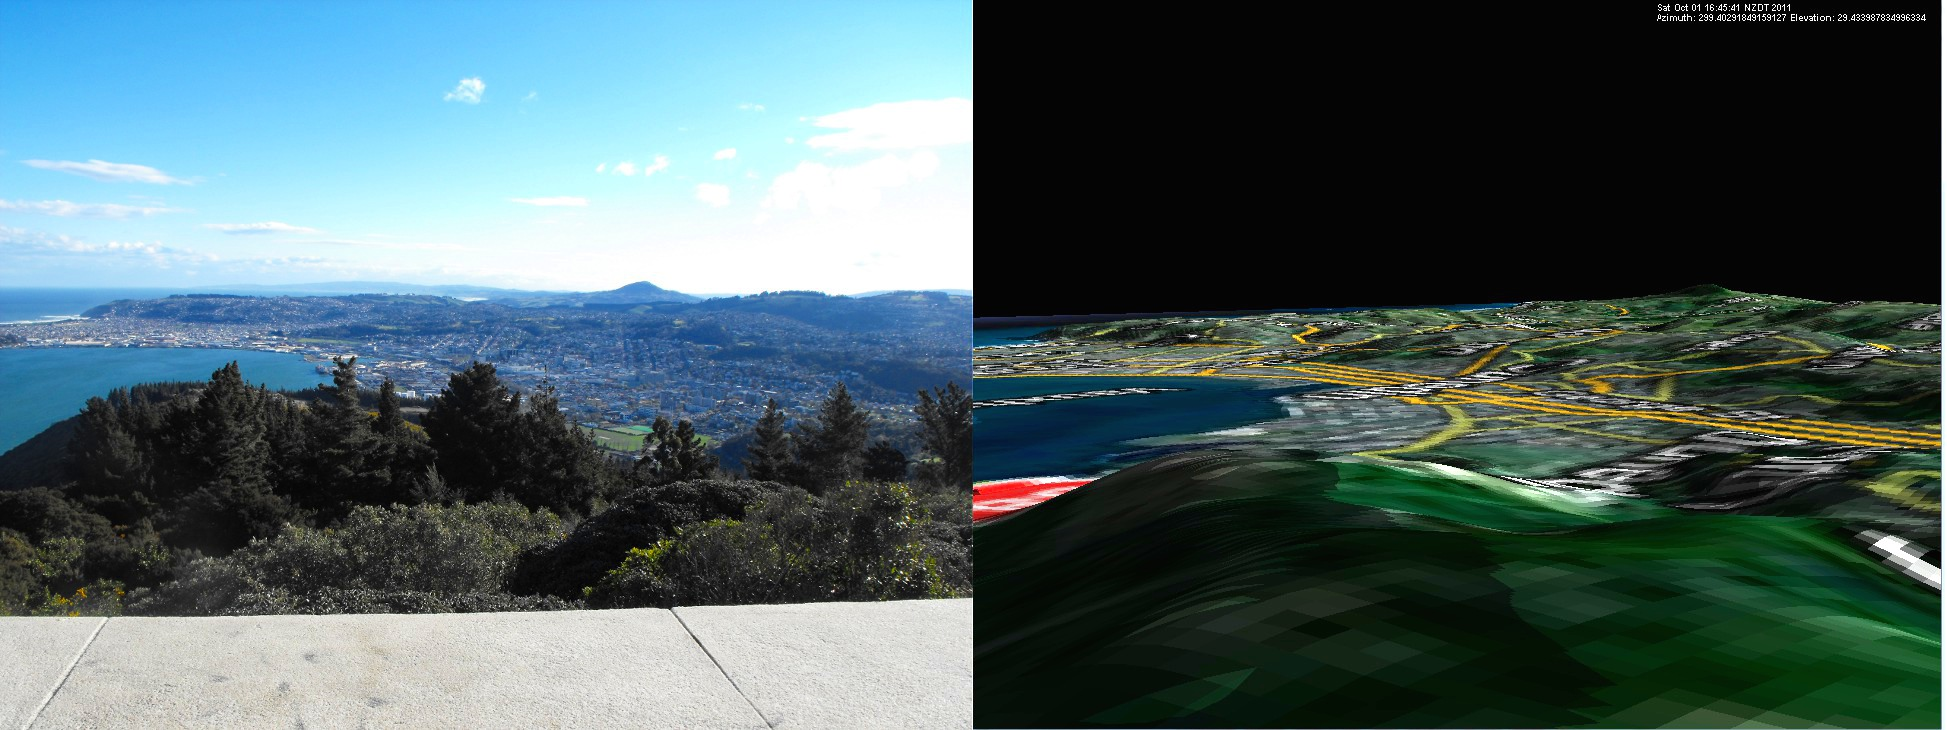
\includegraphics[width=\textwidth]{realvsviewer.jpg}
\caption{A camera image taken from signal hill at 16:45 on September 28th 2011 and the same image generated in the viewer}
\label{image:realvsviewer}
\end{figure}

In figure~\ref{image:realvsviewer} the scene generated by the viewer from the top of signal hill is very similar to that of an actual image. All of the major geographical features of Dunedin can be made out and similar shadows are present in both images. Not seen in the photograph is the position of the Sun, which was in approximately the same position in both scenes. In both scenes shadows can be seem forming around the town belt area and on the hills near St. Clair beach.

\section{Usage}

To run the viewer firstly the JOGL libraries must be installed and set up to work with the installed Java runtime library. Running the OpenGL code requires a graphics card that fully supports OpenGL version 2. See the controls below for an idea of how to run it. Command line parameters are not given.

\subsection{Control}

\texttt{w} $\rightarrow$ Move forward\\
\texttt{s} $\rightarrow$ Move backward\\
\texttt{a} $\rightarrow$ Strafe left\\
\texttt{d} $\rightarrow$ Strafe right\\
\texttt{f} $\rightarrow$ Toggle wireframe mode\\
\texttt{p} $\rightarrow$ Print the current 3D coordinates to stdout\\
\texttt{=} $\rightarrow$ Increase the time speed by one second\\
\texttt{-} $\rightarrow$ Decrease the time speed by one second\\
\texttt{0} $\rightarrow$ Stop time\\
\texttt{h} $\rightarrow$ Move camera position to Signal Hill\\
\texttt{m} $\rightarrow$ Toggle between aggregator shadows and shadow mapping\\
\texttt{g} $\rightarrow$ Start/stop the aggregator updating\\

Mouse drags can be used to rotate the camera up, down, left and right. For example if the user wishes to look to the right they would click and drag the mouse right and the camera will move once they let go of the mouse.

\section{Future Work and Extensions}
Instrumenting the viewer to run a loop based on a script passed into the viewer was on the agenda to implement if there was enough time. This would have allowed the program to give a quick demonstration of how it can be used and what values can be gathered without looking through the documentation. Profiling and testing of the viewer could also be done repeatedly and accurately by running the code through the script and outputting differences and errors between different versions of the software.

\chapter{Data Aggregator for Accurate Shadow Calculation and Data Accumulation}
The aggregator calculates shadows by ray tracing a light ray from a point in the elevation data to the Sun and checking for intersection. It does this on a per vertex basis to ensure each vertex is calculated accurately, unlike OpenGL methods such as shadow mapping which may use the same shadow calculation on multiple vertices, causing artefacts to appear around edge cases. The aggregator can be run as a standalone program where Targa format (TGA) image files and comma separated value (CSV) files are output or as part of the viewer to accurately calculate the shadows.

\section{Cleary's Algorithm for Calculating Shadows}
To calculate whether a given point is in shadow or not a modified version of Cleary's algorithm~\cite{cleary} is used, see algorithm~\ref{alg:shadow-calculation} for a full description. Cleary's algorithm was originally used for fast spacial subdivision, however it works equally well in ray tracing a light ray from a point through a two-dimensional grid of points like the one present in the elevation data. For each point, the light ray travels from the source to the Sun through each grid square it meets until it reaches the end of the grid. At each grid line intersection the height at that point is compared to the height of the Sun along the direction vector between the starting point and the Sun, if the direction vector's $y$ value multiplied by the current position on the direction vector is less than the height at that point then it is said to be in shadow, otherwise it continues on the direction vector to the Sun until the end of the grid is reached or another point causes it to be seen to be in shadow.

\begin{algorithm}[h]
\caption{Calculate whether a given $x,y$ point in the elevation data is in shadow}
\label{alg:shadow-calculation}% and a label for \ref{} commands later in the document
\begin{algorithmic}           % enter the algorithmic environment
\STATE $\mathit{directionToSun} \leftarrow \mathit{sun}.\mathit{directionVector}$
\STATE $\mathit{heightAtPoint} \leftarrow \mathit{map}.\mathit{getHeight}(x,y)$
\STATE $\mathit{tdx} \leftarrow 1 / \mathit{directionToSun}.x$
\STATE $\mathit{tdy} \leftarrow 1 / \mathit{directionToSun}.y$
\STATE $\mathit{xPosition} \leftarrow x$
\STATE $\mathit{yPosition} \leftarrow y$
\WHILE{$\mathit{xPosition} < \mathit{map}.\mathit{width} \wedge \mathit{yPosition} < map.height \wedge \mathit{xPosition} \geq 0 \wedge \mathit{yPosition} \geq 0$}
	\IF{$\mathit{height}(\mathit{xPosition},\mathit{yPosition}) \times |\mathrm{max}(tdx,tdy)| > \mathit{directionToSun}.y\times |\mathrm{max}(tdx,tdy)|$}
		\RETURN{\texttt{In Shadow}}
	\ENDIF
	\IF{$|tdx| < |tdy|$}
		\STATE $dx \leftarrow 1 / \mathit{directionToSun}.x$
		\IF{$tdx > 0$}
			\STATE $\mathit{xPosition} \leftarrow \mathit{xPosition} + 1$	
		\ELSE
			\STATE $\mathit{xPosition} \leftarrow \mathit{xPosition} - 1$	
		\ENDIF
		\STATE $tdx \leftarrow tdx + dx$
	\ELSE
		\STATE $dy \leftarrow 1 / \mathit{directionToSun}.y$
		\IF{$tdy > 0$}
			\STATE $\mathit{yPosition} \leftarrow \mathit{yPosition} + 1$	
		\ELSE
			\STATE $\mathit{yPosition} \leftarrow \mathit{yPosition} - 1$	
		\ENDIF
		\STATE $tdy \leftarrow tdy + dy$		
	\ENDIF
\ENDWHILE
\RETURN{\texttt{Not In Shadow}}
\end{algorithmic}
\end{algorithm}

\section{Integration Into the Viewer}
The aggragator output can be run in the viewer if the `use aggregator' and `generate aggregator texture' switches are turned on. The aggregator works in the viewer by generating a texture out of the current shadow information, with pixels coloured white for not in shadow and black for in shadow. By placing the texture over the map of Dunedin aggregator shadows can be observed on the terrain. Because the aggregator uses different shader programs to the viewer, overlay images and shading are not drawn on the scene.

\section{Picking the Areas to Scan}
The aggregator uses the overlay image seen in figure~\ref{image:elevation-water} to select which points to scan. Any area that is coloured a strong blue is counted as in water and any area that is a solid black colour is thought of being outside the desired range to scan and can be left out of the aggregator calculations. This allows the user to specify specific areas of Dunedin that they wish to ignore, by painting them black or blue. The aggregator can be run faster through this method because the points do not need to be checked for shadows, giving a linear speed increase in the number of points ignored. Data output from ignored areas is presented as a black square when outputting to a Targa file or as a value with no contents in a CSV file.

\section{Optimisations}
The aggregator runs fastest when there are a large number of shadows cast over the city, allowing it to break out of the shadow-tracing algorithm early. When there are few shadows being cast the runtime of the aggregator slows down by a large factor because it has to scan to the edge of the map for every point to find if it is not in shadow. During solar noon, when most of the scene is in sunlight, the aggregator runs at its slowest because the highest number of points shadow trace to the edge of the map.

By subdividing the map into small areas and checking for shadows around the edge of each area the aggregator can run faster when there are large sections of the scene that receive direct sunlight. If there is no shadow present around any of the edges and the area is reasonably flat (no more than five metres of variation around the edges) then it is safe to assume that all of the points within that region will not be in shadow. The aggregator uses a square area of 10 points which it scans around the outside edge of for shadows, if no shadow is found then all of the points within the square are set to be not in shadow, otherwise it na\"{\i}vely scans all of the points within the region for shadows.

\subsection{Speed Increase}
\begin{figure}[h]
\centering
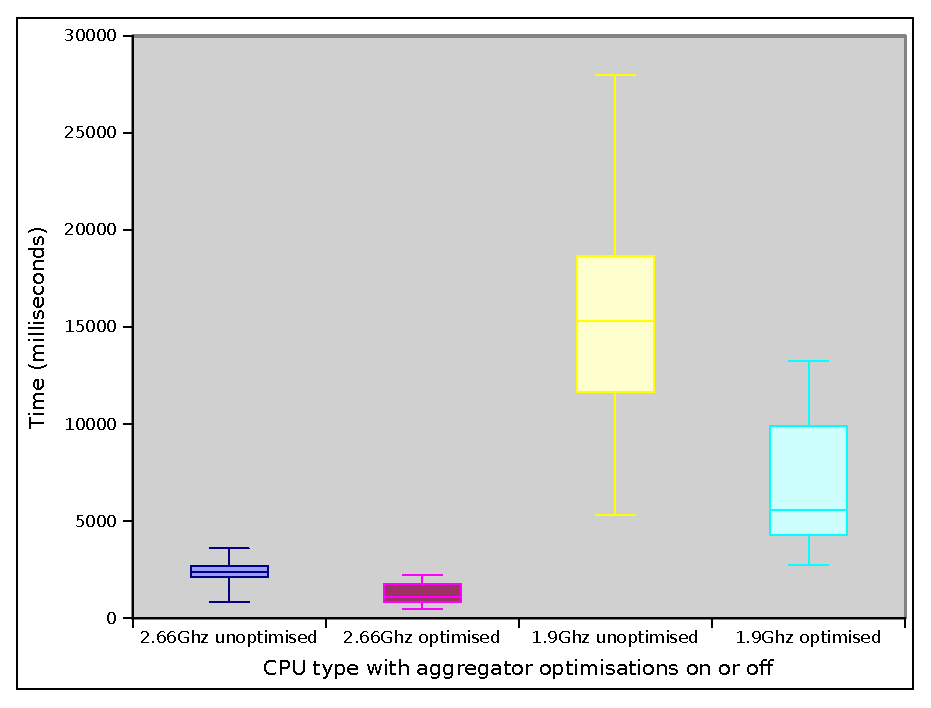
\includegraphics[width=\textwidth]{aggregator-optimisations-graph.eps}
\caption{Time taken to run the aggregator between the times of 08:00:00 and 17:59:24}
\label{image:aggregator-optimisations-graph}
\end{figure}

To test the effect of the edge scanning optimisation the data aggregator was run 1000 times on two different computers for the whole of Dunedin (ignoring only water) between the times of 08:00:00 and 17:59:24 on October 1st 2011, with the average time in milliseconds it took to run the shadow-tracing over the entire scene recorded at each time. On a 1.9GHz AMD Dual Core Turion processor the optimised code took an average of 6800.486 milliseconds and the unoptimised code took 15977.598 milliseconds to calculate all of the shadows at a given time. Using a 2.66 GHz Intel Core i7 920 processor the optimised code took an average of 1147.176 milliseconds and the unoptimised code took 2551.007 milliseconds to calculate the shadows. Using the optimised code increased the speed by a factor of 2.35x on the 1.9GHz processor and 2.19x on the 2.66GHz processor. The graphed results of this experiment can be seen in figure~\ref{image:aggregator-optimisations-graph}, with the standard deviation, mean and extreme number of milliseconds the aggregator took to run over the entire city at different times of the day.

\subsection{Other Methods}
The code does not necessarily need to be linearly optimised to speed it up. With multi-core processors becoming more common on computers, multi-threading the shadow-tracing code to take advantage of more than one processor at a time would give significant performance increases because the calculation of the shadows for each point does not depend on the state of any other point at a fixed time. Threading the data can be accomplished subdividing the data into work units, queuing the work units to be processed and waiting for each unit to finish which should give a increase in computation time relative to the number of processing cores.

\section{Comparison to OpenGL Shadow Mapping}
\begin{figure}[h]
\centering
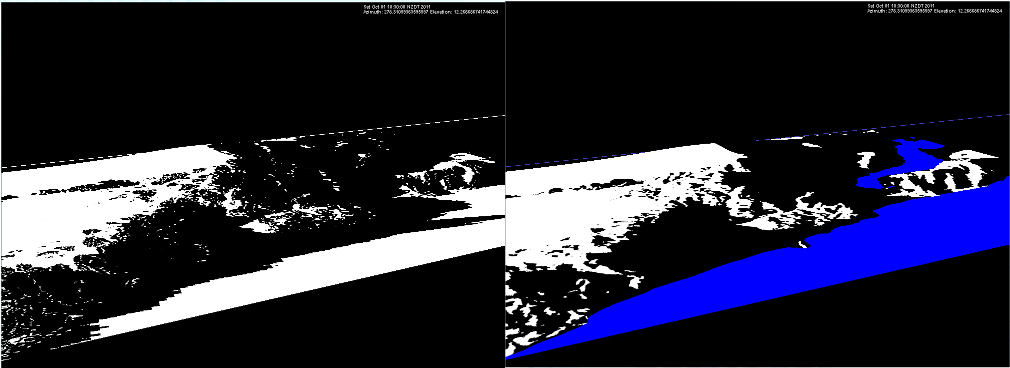
\includegraphics[width=\textwidth]{aggregatorvsshadowmapping.png}
\caption{A side-by-side screenshot comparison of shadowing using shadow mapping (left) and shadow tracing (right)}
\label{image:aggregatorvsshadowmapping}
\end{figure}

Shadow maps are noticeably less accurate at calculating shadows then the shadow-tracing methods the aggregator uses. In the side-by-side comparison in figure~\ref{image:aggregatorvsshadowmapping} it can be seen that shadows generated by shadow mapping have noticeable aliasing and calculation errors. Aliasing around the edges of shadows occurs in the shadow map when the angle between the Sun and the map of Dunedin approaches 180{\degree} and the shadows begin to grow long. Self-shadowing is also a problem with shadow mapping and can only be fixed by increasing the accuracy of the depth buffer. Neither of these problems arise in the data aggregator because of the accuracy gained by shadow-tracing the area between the shadow and the Sun and checking for intersections. The aggregator pays for this accuracy by running slower than real-time (approximately 7 seconds between calculations for an older 1.9GHz machine and 2.5 on a newer 2.66GHz machine) compared to the shadow maps which run at $>$30 calculations/second with a dedicated graphics processor.\note{I'm not going to make accurate estimations about how fast the viewer runs because the speed difference between different graphics processing units is quite large}

\note{why would frame skipping be performed? The time is updated every frame not the other way round, by real-time I mean the program updates more than 24 times per second}\notedme{Where does 24 come from?? Heh heh - I should really have asked earlier about your take on time, as I think there's something I don't understand about it (although it's obviously not much of a problem!). One fundamental point is that if you can generate a graphics frame in less time than it takes to display it, then you probably don't need to optimise your code further for interactive use. I'd expect most monitors these days update at rates between 60Hz and 120Hz. I wouldn't see a need to link simulation time with wall-clock time, as presumably this is not going to be informative for interactive use (a nice screen saver idea, though). In the above discussion of ``real-time'', though, assuming that you wanted to link simulation-time with wall-clock time, surely you would just set simulation-time to step in the same way wall-clock time does with every frame (i.e. 7s on the old machine). Hmm, OK, I think I've talked myself around to seeing what you are saying. I think you mean slower than ``convenient for interaction'' rather than ``real-time'' I think - so 24fps is your estimate of the eye's perception of frame update speed?}\note{yes. I've added a footnote in the introduction to make this distinction.}

\section{Output}

\begin{figure}[h]
\centering
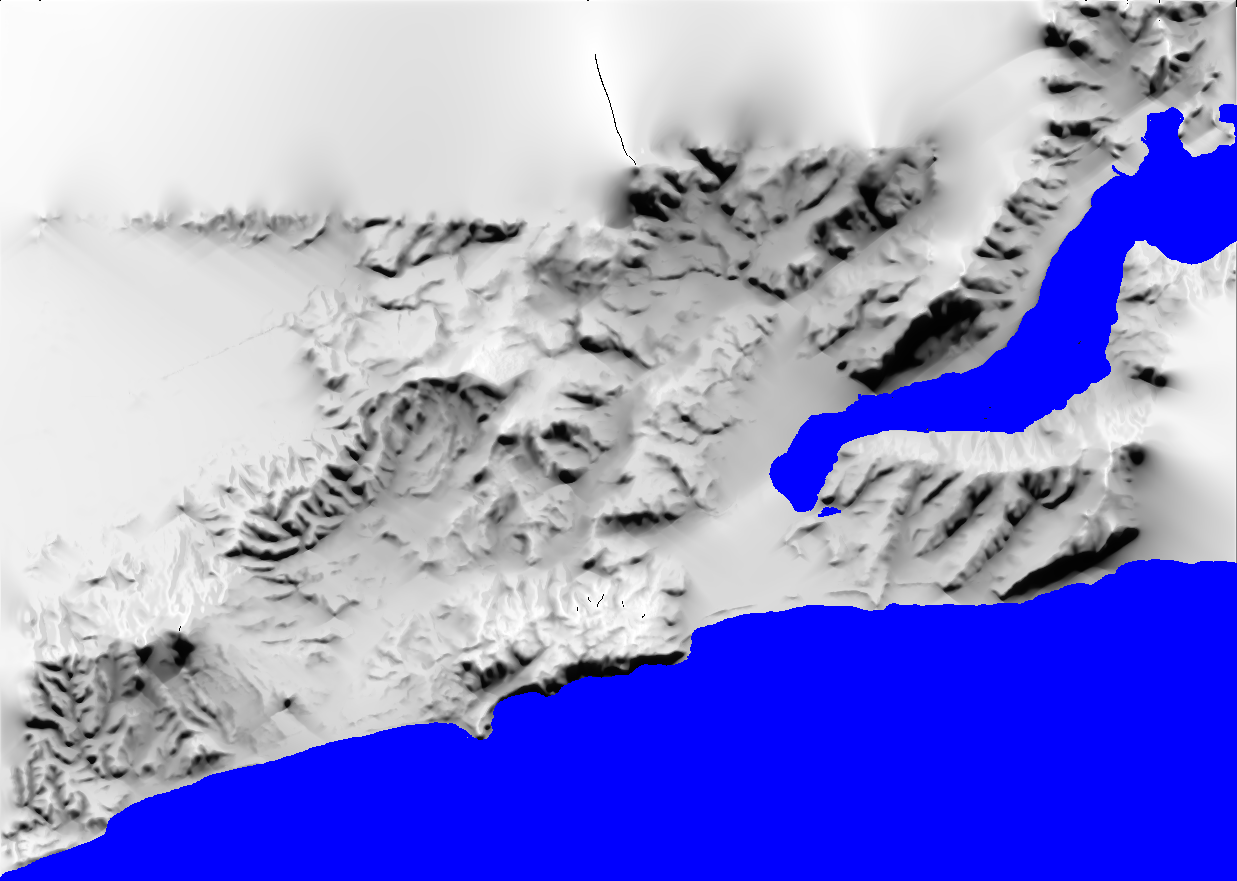
\includegraphics[width=0.8\textwidth]{june.png}
\caption{Distribution of sunlight for the month of June 2011}
\label{image:aggregator-targa-output}
\end{figure}

\notedme{This figure is fantastic! :-)}
When the aggregator is run as a standalone program a Targa image file and a comma separated value (CSV) file will be created. When simulated over a given period of time , for example October 4th 2011 to November 14th 2011,\notedme{not clear if you mean simulation time or wall-clock time - obviously simulation time}\note{fixed} the program will output a CSV file with the seconds-of-sunlight received for every point and a Targa image with a linear scale between areas that received the lowest levels of sunlight in black and the areas that received the most sunlight in white.\notedme{linear scale? if so, say so}\note{fixed}

\subsection{Interpretation of the Seconds-of-Sunlight Data}
\begin{figure}[h]
\centering
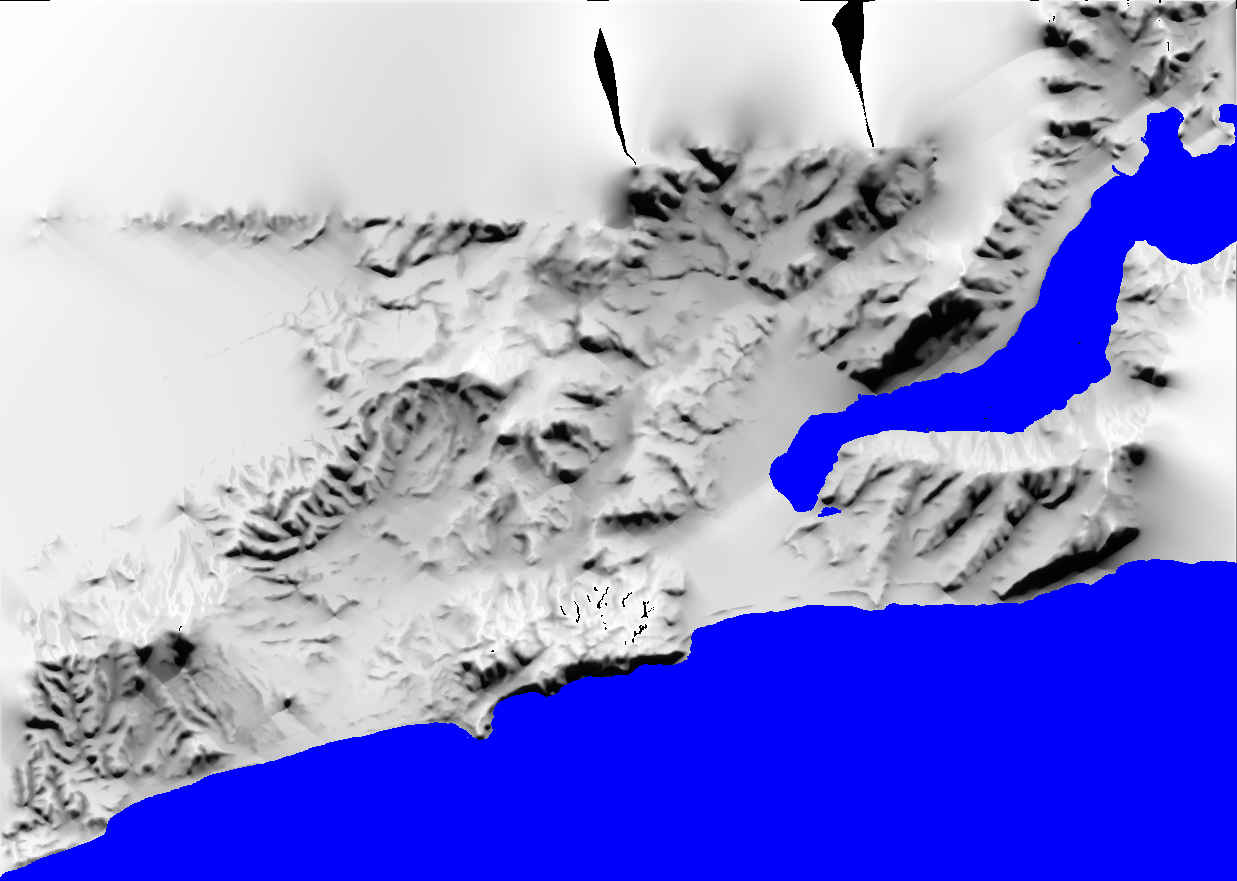
\includegraphics[scale=0.25]{wintersolstice.png}
\caption{Total sunlight received on June 21st 2011 (winter solstice) between 08:25 and 16:45}
\label{image:wintersolstice}
\end{figure}

Certain areas of Dunedin such as Leith Valley, the town belt and the west side of north-east valley are well known for receiving the lowest levels of sunlight in Dunedin. In figure~\ref{image:aggregator-targa-output}, showing the distribution of sunlight over the month of June, it can be seen that the distribution of sunlight was far lower in areas that were on or nearby the south facing side of a hill. Areas that received the largest distribution of sunlight were either far away from any hills, such as South Dunedin, or on the north facing side of a hill, such as the peninsula.

\section{Accuracy}
Differences between real world sunlight distribution and that generated by the aggregator will be different depending on the land usage. The height data used in the project and the interpolation between points assumes that the area is completely flat, however in areas containing large buildings and/or tall trees the height of the shadows cast from the area could be 10-40 metres higher than ground level. The only way to approximate around this would be to classify the height above sea ground\notedme{?} level depending on the usage of the land. For example the central business district will contain scatterings of large buildings casting shadows 20-40 metres higher than ground level and a forested area will cast shadows 5-70 metres higher than ground level.

\section{Future work}
With more time more complicated optimisations could have been explored. For example, shadow backtracking
finds points in shadow and assumes that nearby points in the direction of the sun that are lower than or equal in height to the current point will be in shadow. Common points that cause shadows such as the ridge line of a hill could potentially be stored and intersections with these points checked before na\"{\i}vely checking for intersections with every point. Threading the code would also provide a great speed increase if the computer it is running on has more than one CPU core, given that the shadow-tracing algorithm has no data interdependencies between different points.\notedme{you need to justify this by saying that you know the data is separable. Some software has data dependencies that means multi-core systems won't speed it up.}\note{this is stated earlier in the section but I'll add it again here}

\notedme{Did the ``suburb'' masking code end up making it? I don't think the figures show anything but sun over the whole area. It would be great to have a table that shows a quantitive difference between Peninsula and North Valley sunlight over June, for example. Even if the code was nearly ready but not finished, it might be worth mentioning it, as being able to quantitatively compare the amount of sun between selected areas of the map would be a good extension.}
\note{Part on the suburb masking code}

\subsection{Sunlight Comparisons Between Suburbs}

The ability to find the average amount of sunlight different suburbs receive was part of the original proposal and almost made it into the project. Currently suburbs can be compared by running the aggregator over a section of Dunedin by blacking out the areas in the terrain map (the map that defines what is water, what is land and what areas should be ignored) that are not in the suburbs to be compared. These suburbs can be compared by exporting this data to a CSV file and calculating the total and average amount of sunlight seconds each suburb received. Originally the output from the aggregator was going to have a different output method that would give the total and average amount of sunlight received for a given suburb overlay map (where suburbs are coloured differently). Unfortunately creating the suburb map was difficult because the distinction between what areas are in what suburb are difficult to make and there simply was not enough time to program the output from the aggregator to give detailed suburb information.

\chapter{Conclusion}
The project managed to accomplish more than what it set out to achieve by creating the interactive three-dimensional display that shows real-time distribution of sunlight over the city of Dunedin and a data aggregator that can augment the display with computed measures of sunlight coverage over time ranges and output them to files. 

\section{Changes Between the Proposal and the Final Report}
Slight modifications were made to the original project proposal: using a global positioning system to check the accuracy of the height information was not used, exporting the height data into a format readable by three-dimensional modelling software not not used, the viewer ended up being a real-time application instead of showing point in time distributions and the aggregator can not only display computed measures of sunlight over time ranges it can also be run as a more accurate alternative to the OpenGL shadowing code.\notedme{Yep - good stuff! :-)}

\section{Physical Data}
Geographical information about the city of Dunedin was collected from multiple sources. The height data came from the surveying department, a map overlay was created using an image from Google Maps~\cite{gmaps} and the position of the sea was generated by hand. While it was difficult to prove the accuracy of the elevation data without the correct tools or sources, comparing real-world images with the physical data showed a relatively close mapping between the data collected and the physical world.

Finding the Sun's position at a given point in time required trial and error before calculations were found that generated accurate results. The Java Sun position library~\cite{javasunlib}, and many other Sun position calculations, use calculations such as the PSA~\cite{psa} and SPA~\cite{spa} algorithm that do not work in the southern hemisphere\cite{southsun}. Code from the Redshift project~\cite{redshift} and calculations from The University of Southern California Department of Architecture~\cite{solarazi} were integrated into a solar positioning library and used to calculate the solar elevation and azimuth at a given time. By testing the calculations generated against other calculations and the real world position of the sun, the accuracy of the Sun's position was validated.

%The most useful extension to this project would be to allow it to work on data sets outside of the the city of Dunedin. With the code already there to calculate the Sun's position all it would take is a way of gathering more elevation data and the project could be expanded to calculate the Sun interaction with a far greater area, or as a way of comparing and contrasting the sunlight cities receive. 

\section{Viewer}\note{Should I change these headings?}
The viewer grew from a simple tool designed to show point in time calculations of the distribution of shadows over the city of Dunedin into a fully fledged OpenGL program that can render shadows in real-time, allow the user to position the camera anywhere in the scene, view output from the aggregator and modify the time speed. Using OpenGL buffers to quickly transfer the vertex and texture data to the graphics processing unit and GLSL shaders to render user-programmable lighting effects such as shadow mapping, the viewer is able to efficiently and quickly render the scene.

\section{Aggregator}
Using a modified version of Cleary's algorithm~\cite{cleary} to calculate intersections through a two-dimensional grid of data it is possible to calculate if a point is in shadow. This is performed by stepping a simulated light ray along the direction vector to the sun through the grid and checking if the point on the grid was higher than the position of the Sun, if so then it is in shadow, if not the algorithm continues until the end of the grid is reached. Shadows generated by the aggregator's shadow-tracing algorithm are noticeably more accurate than those generated using OpenGL shadow mapping, for example in figure~\ref{image:aggregatorvsshadowmapping} the shadow mapping code contains artifacts and self shadowing while the aggregator exhibits none of these traits.

The aggregators shadow-tracing calculation can be optimised when the Sun's elevation is high by subdiving the scene and checking for shadows around the edge of the subdivision. If a shadow is not found around the edge of the subdivided area then can be assumed that no point within that area will be in shadow. Otherwise, if a shadow is found then each point in the subdivision is na\"{\i}vely checked to see if it is in shadow. Using this optimisation the aggregator was shown to run, on average, more than two times faster when compared to the unoptimised code path.\note{rewrote this part}

Aggregate information showing the distribution of sunlight over a period of time such as that seen in figure~\ref{image:aggregator-targa-output} confirmed the theory that certain parts of Dunedin receive far less sunlight than others. It can be seen from figures~\ref{image:aggregator-targa-output} and \ref{image:wintersolstice} that the areas that received the largest amount of sunlight were on north facing hills such as the Penesula, areas on the south face of hills such Ravensbourne received little to no sun and areas that are not surrounded by hills such as Mosgiel and South Dunedin receive moderate amounts of sunlight.\notedme{figure references are broken in this paragraph (they shouldn't all be the same)}\note{oops didn't notice this when I was changing some images around}

\bibliographystyle{abbrv}
\bibliography{480}

\end{document}
